% ------------------------------------------------------------------
% Fellowship proposal -- science core (v0.4, 2 Sept 2026; post second review)
% Author: Dylan J. Gormley
% Build: pdflatex main.tex  (twice, for references)
%
% This file is the single source for every application:
%   NHFP  = Sections 1-7 (Research Proposal) + Section 8 (Previous and
%           Current Research); 8 pages total incl. figures, 12 pt, 1 in.
%   KICP  = Sections 1, 3, 5 compressed to 1-3 pages.
%   AAPF  = Sections 1-7 + education plan + host justification + career
%           goals (separate file), 10 pages, with a "Broader Impacts"
%           header on its own line.
% Red bracketed text = to be filled or verified before submission.
% ------------------------------------------------------------------
\documentclass[12pt]{article}
\usepackage[margin=1in]{geometry}





\usepackage{mathptmx}
\usepackage{amsmath,amssymb}
\usepackage{graphicx}
\graphicspath{{./figs/}}
\usepackage{xcolor}
\usepackage[font=small,labelfont=bf]{caption}
\usepackage{enumitem}
\usepackage{array}
\usepackage{float}
\usepackage[hidelinks]{hyperref}
\hypersetup{pdftitle={A Cyclostationary Estimator for Discrete-Delay Instrument Systematics in 21 cm Cosmology with CHIME and CHORD},pdfauthor={Dylan J. Gormley}}
% Let floats pack tightly; with three figures in eight pages the default
% topfraction/textfraction leave half-empty pages.
\renewcommand{\topfraction}{0.92}
\renewcommand{\bottomfraction}{0.75}
\renewcommand{\textfraction}{0.06}
\renewcommand{\floatpagefraction}{0.80}
\setcounter{topnumber}{2}
\setlength{\parskip}{0.35em}
\setlength{\parindent}{0pt}
\newcommand{\todo}[1]{\textcolor{red}{[#1]}}
\newcommand{\hMpc}{\,h\,\mathrm{Mpc}^{-1}}
\newcommand{\kpar}{k_\parallel}
\newcommand{\kperp}{k_\perp}
\newcommand{\cyl}{\mathrm{CHIME}}
\setlist{nosep,leftmargin=1.2em}

\begin{document}

\begin{center}
{\large\bfseries A Cyclostationary Estimator for Discrete-Delay Instrument Systematics in 21\,cm Cosmology with CHIME and CHORD}\\[0.4em]
Dylan J.\ Gormley \quad (West Virginia University; proposed host: \todo{University of Chicago / KICP, sponsor TBD})
\end{center}

\section*{Research Proposal}

\subsection*{1. Science Objective and Current Limitation}

Redshifted 21\,cm intensity mapping measures neutral-hydrogen clustering over volumes and redshifts that galaxy surveys sample sparsely, with systematics distinct from optical spectroscopy. The baryon acoustic oscillation (BAO) feature constrains $H(z)\,r_d$ and $D_A(z)/r_d$, while redshift-space anisotropy constrains $f\sigma_8$. The 400--800\,MHz band of the Canadian Hydrogen Intensity Mapping Experiment (CHIME) spans $0.8<z<2.5$~\cite[Abstract; Sec.~I; Fig.~1]{chime2022}. It overlaps the quasar and Lyman-$\alpha$ samples of the Dark Energy Spectroscopic Instrument (DESI)~\cite[Sec.~2.2; Table~1]{desi2024} and the planned $z=1$--2 H$\alpha$ survey of the Nancy Grace Roman Space Telescope~\cite[Abstract]{roman2021}. A BAO measurement would therefore provide a complementary dark-energy probe with largely independent instrumental systematics.

Recent CHIME measurements motivate this work. Following cross-correlation detections with galaxy surveys~\cite[Abstract]{chime2023} and the Lyman-$\alpha$ forest~\cite[Abstract; Sec.~VI.2; Table~1]{chime2024lya}, the collaboration measured the 21\,cm auto-power spectrum at $z\simeq1$ with a new pipeline~\cite[Abstract; Table~2]{chime2025auto}. The $12.4\sigma$ result uses 94 nights over 608--708\,MHz and $0.4\lesssim k\lesssim1.5\hMpc$. It is CHIME's first large-scale-structure measurement at this redshift without an external catalog and constrains $\mathcal A_{\rm HI}$ with phenomenological small-scale shape terms~\cite[Secs.~6.2.1 and 6.2.3; Eqs.~(74)--(75), (78)]{chime2025auto}.

However, this result does not yet constrain the BAO scale. The pipeline applies the DAYENU inverse-covariance high-pass filter~\cite[Sec.~3.2; Eqs.~(21)--(25)]{dayenu} with a CHIME-specific cutoff of 200\,ns~\cite[Sec.~3.2.3; Eqs.~(15)--(18)]{chime2025auto}. It then discards line-of-sight modes below 280\,ns, where the filter response has not recovered, and the published measurement begins at $\kpar=0.35\hMpc$~\cite[Sec.~5.3; Eq.~(64); Fig.~10]{chime2025auto}. Because every mode with $|k|<0.35\hMpc$ also has $\kpar<0.35$, this filtering removes all BAO-scale modes at $k\simeq0.05$--$0.3\hMpc$. At $z=1.16$, these modes correspond to delays of roughly 40--240\,ns (Fig.~\ref{fig:budget}). The published auto-spectrum therefore constrains the signal amplitude, but the filtering removes the modes required for a BAO measurement~\cite[Sec.~3.2]{chime2025auto}.

The first objective is to determine what occupies the discarded 100--280\,ns window. The collaboration expects foregrounds in the beamformed data, including instrumental chromaticity, to remain below roughly 200\,ns. The current analysis associates this chromaticity with mutual coupling and reflections in the analog chain, whose periodic bandpass structure is set by the telescope's physical and electrical length scales~\cite[Sec.~3.2; Sec.~3.2.3, Eqs.~(15)--(18)]{chime2025auto}. It also subtracts a daily estimate of additive cross-talk~\cite[Sec.~3.5.2; Eq.~(27)]{chime2025auto}.

Several known mechanisms produce discrete delays. A standing wave in the $\sim$5\,m feed--reflector cavity produces a 30\,MHz ripple, or 33\,ns delay, whose peaks shift with declination~\cite[Sec.~V; Figs.~4--5]{chime2024holo}; the daily Cygnus~A calibration imprints this structure on all data~\cite[Fig.~5]{chime2025auto}. Cross-talk may extend to the 78\,m instrumented cylinder length, corresponding to a one-way light time of $\sim$260\,ns~\cite[Appendix; Table~2]{chime2022}. The current analysis also documents a 50\,m cable with a 390\,ns round-trip reflection~\cite[Sec.~7.9]{chime2025auto}. It has not yet been established how much of the 100--280\,ns power is concentrated at discrete delays, rather than distributed through smooth chromaticity or the geometric wedge. This proposal tests the hypothesis that \emph{discrete delays dominate the reclaimable part of the window}. The statistic in Section~3 provides this test on existing data, and the result is the first decision gate in Section~5.

If the hypothesis holds, I will proceed in three steps. First, I will use the foregrounds to detect discrete delays above a calibrated threshold. Next, I will estimate a low-parameter model for each delay by declination and transit, then remove it with a delay-shift canceller. Finally, I will certify the correction with false-alarm calibration, split-sample estimation, signal injections, and a residual budget expressed as BAO parameter bias. The split removes noise bias, while injections measure signal-correlated loss because both halves share the same sky. These tests determine the certified foreground cut. I have applied cyclostationary signal processing (CSP) to communications signals and National Aeronautics and Space Administration (NASA) spectrum sensors for fifteen years, and my CHIME baseband dissertation provides the required pipelines.

Figure~\ref{fig:taucut} gives the numerical requirement. Using published CHIME parameters, a Fisher forecast reaches a $5\sigma$ BAO-amplitude detection for the seven-year archive when $\tau_{\rm cut}\simeq100$--$140$\,ns, depending on sky area, or $\simeq150$\,ns when the filter's soft transition is included. The $3\sigma$ range is $\simeq110$--$150$\,ns, while the present 280\,ns floor retains essentially no BAO sensitivity. Archive duration, full-band processing, and sky area are collaboration plans rather than proposal deliverables; Section~4 separates these dependencies.

\begin{figure}[htbp]
\centering
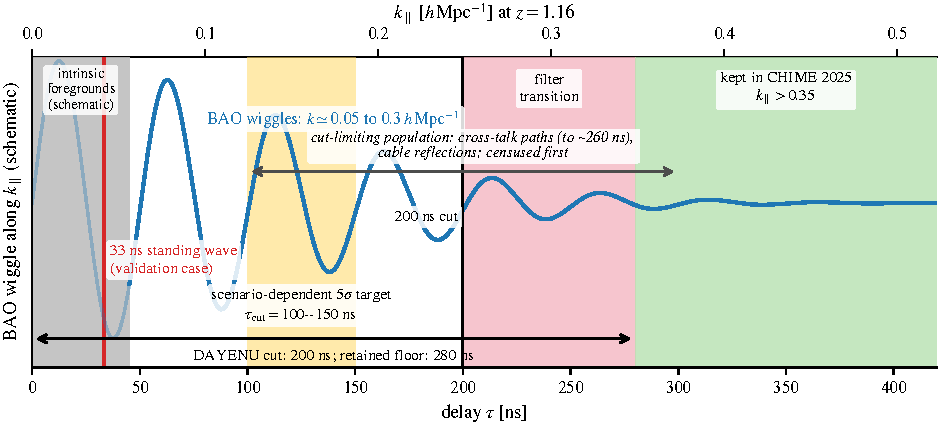
\includegraphics[width=\textwidth]{fig_delay_budget.pdf}
\caption{Delay budget for the CHIME 21\,cm auto-spectrum analysis at $z=1.16$~\cite[Sec.~5.3; Eq.~(64); Fig.~10]{chime2025auto}. The BAO feature is shown schematically along $\kpar$ for the $\mu=1$ projection. Because $|k|\ge\kpar$, the $\kpar<0.35$ cut removes all BAO-scale modes, not only radial modes. The pipeline retains delays above 280\,ns (green). The discarded window contains the BAO feature (blue), the 33\,ns standing wave used for validation (red)~\cite[Sec.~V; Figs.~4--5]{chime2024holo}, and, if the hypothesis in Section~1 is correct, the longer cross-talk and cable delays that limit the cut. The yellow band shows the scenario-dependent $5\sigma$ target from Fig.~\ref{fig:taucut}. The grey region illustrates intrinsic foreground support on a short baseline; it is schematic, and intrinsic foregrounds cannot be recovered by this method.}
\label{fig:budget}
\end{figure}

\subsection*{2. Physical Model and Existing Pipeline}

We begin by modeling the beamformed visibility for one polarization, east--west baseline, declination bin, and 9.94\,s integration as
\begin{equation}
d(\nu) \;=\; \bar g(\nu)\Big[1 + \sum_{k=1}^{K} \epsilon_k\, e^{\,2\pi i \nu \tau_k}\Big]\, s(\nu) \;+\; \sum_{j} c_j\, e^{\,2\pi i \nu \tau'_j} \;+\; n(\nu),
\label{eq:model}
\end{equation}
where $s(\nu)=F(\nu)+h(\nu)$ contains the foregrounds $F$ and the 21\,cm signal $h$, with $F\sim10^4$--$10^5\,h$. The quantity $\bar g$ is the smooth gain, $\{\tau_k,\epsilon_k\}$ are the delays and complex amplitudes of multiplicative reflections, $\{\tau'_j,c_j\}$ describe additive cross-talk paths, and $n$ is noise. After calibration, we absorb the residual smooth gain into $S$. The corresponding idealized delay-domain model is
\begin{equation}
D(\tau) \;=\; S(\tau) + \sum_k \epsilon_k\, S(\tau - \tau_k) + \sum_j c_j\, \delta(\tau-\tau'_j) + N(\tau).
\label{eq:delay}
\end{equation}
The foreground occupies $|\tau|\lesssim\tau_F$, where $\tau_F$ depends on baseline and direction. Its support extends from a few tens of nanoseconds for main-lobe emission on short baselines to the horizon delay $b/c\simeq220$\,ns for far-sidelobe sources on the 66\,m baselines. A reflection copies the foreground structure carried by a baseline to $\tau_k$ with attenuation $|\epsilon_k|$. The copy is compact on short baselines and broad where the wedge is broad. An additive cross-talk path is an impulse in the infinite-band idealization. A finite band and taper broaden it into a localized kernel. Both effects remain localized in delay and periodic in frequency.

The existing pipeline treats these terms in several stages. First, DAYENU strongly attenuates modes below $\tau_{\rm cut}=200$\,ns, with the loss of low-$\kpar$ modes described above. Next, additive cross-talk is estimated separately for each sidereal day, polarization, channel, east--west baseline, and north--south position. The estimator uses weighted medians of the real and imaginary visibilities over a quarter-specific, one-hour interval in local Earth Rotation Angle (ERA)~\cite[Sec.~3.5.2; Eq.~(27)]{chime2025auto}. This subtraction removes the component that is stable within the reference interval, but retains drift and sky-dependent structure. It also does not correct multiplicative terms, which track the sky.

The pipeline then applies the general Hybrid Foreground Residual Subtraction (HyFoReS) cross-correlation estimator~\cite[Sec.~III.A; Eqs.~(5), (9), (11), pp.~3--4]{hyfores}. HyFoReS estimates one coefficient $\delta g_{pfe}$ per polarization, channel, and baseline by cross-correlating high-pass data with a low-pass foreground template, averaging over the sky, and fitting each day independently~\cite[Sec.~3.3; Eq.~(23)]{chime2025auto}. In simulations, it reduces the bias from $10^{-5}$--$10^{-4}$ bandpass errors mostly below thermal noise. Errors of $10^{-3}$--$10^{-2}$ can be suppressed by roughly three orders of magnitude, with the remaining performance limited by gain-estimation noise and second-order terms~\cite[Secs.~IV.A--IV.B; Figs.~2 and 4, pp.~8--11; Sec.~V.B, p.~14]{hyfores_sim}. On data, the collaboration reports a modest reduction~\cite[Sec.~3.3; Eq.~(24); Fig.~3]{chime2025auto}.

With one free coefficient per channel, HyFoReS averages over declination and time to control the noise of approximately 256 parameters. However, the peaks of the dominant ripple shift with declination~\cite[Sec.~V; Fig.~5]{chime2024holo}. If its phase also varies, a sky average can partially cancel the component being fitted. The proposed method is a sparse-delay extension motivated by HyFoReS. It uses up to $3K$ real parameters for each declination and transit when both the delay and complex amplitude of every term are fitted locally. I will compare the two methods on the same data using parameter count, signal loss, residual bias, and computation. The HyFoReS authors are coauthors on the data I have requested.

Two comparisons establish the expected performance. The 2023 stacking analysis used cuts of order 200\,ns that varied with polarization and declination~\cite[Sec.~IV.5; Eqs.~(53)--(57); Fig.~9; Sec.~V.1, Fig.~13]{chime2023}. That analysis cross-correlated CHIME data with an external catalog, so residuals uncorrelated with the catalog average away. The auto-spectrum has no corresponding immunity, and lowering its cut therefore requires the leakage to be removed. The Hydrogen Epoch of Reionization Array (HERA) uses the same physical model but estimates narrow reflection delays and amplitudes from autocorrelation delay spectra~\cite[Sec.~3.1; Fig.~3, pp.~7--8]{kern2019}, then applies antenna corrections to cross-correlations~\cite[Sec.~3; Fig.~5, pp.~5--8]{kern2020}. The proposed method instead identifies delays blindly from the coherence of cross-correlation data.

\subsection*{3. Cyclostationary Delay Estimation}

A process modulated by a periodic function is cyclostationary. Its spectral correlation function compares components separated by a \emph{cycle frequency} $\alpha$ and can be nonzero when $\alpha$ corresponds to a periodic component. In contrast, stationary noise has no such component at $\alpha\ne0$~\cite[Sec.~3.2.1; Eqs.~(3.6)--(3.11), (3.19), pp.~643--645; Sec.~3.7, Eqs.~(3.88)--(3.95), pp.~651--652]{gardner2006}. More generally, second-order cyclostationary statistics can identify an unknown multipath channel without training data~\cite[Abstract, p.~340; Secs.~I.B--I.C; Eqs.~(1)--(2), p.~341]{tong1994}.

My M.S.\ thesis implemented a low-memory, streaming form of this estimator~\cite[Abstract, p.~vii; Sec.~3.2, pp.~27--29]{gormley2021thesis}. I then implemented the estimator in a field-programmable gate array (FPGA) spectrum sensor at NASA Glenn~\cite[Sec.~II; Figs.~7--9, p.~3; Sec.~III, Table~II, pp.~3--4]{gormley2021}, and later developed a hybrid memory--throughput architecture~\cite[pp.~34--36]{gormley2023}. My dissertation applies first-order periodicity to the Advanced Television Systems Committee (ATSC) pilot. Under the adopted signal and noise model, the corresponding detector is a tone matched filter. That work provides the certification methods used here~\cite{gormley2026a}.

Equation~(\ref{eq:model}) has the same mathematical form after interchanging the axes. Frequency $\nu$ takes the role of time, delay $\tau$ takes the role of frequency, and a reflection at $\tau_k$ becomes a periodic modulation with cycle ``frequency'' $\tau_k$. I therefore define the \emph{delay--offset correlation}
\begin{equation}
C(\tau, \Delta) \;=\; \big\langle D(\tau)\, D^{*}(\tau-\Delta) \big\rangle, \qquad
\gamma(\tau,\Delta) \;=\; \frac{C(\tau,\Delta)}{\sqrt{\langle |D(\tau)|^2\rangle\, \langle |D(\tau-\Delta)|^2\rangle}},
\label{eq:coh}
\end{equation}
where the average is taken over integrations within a transit at fixed declination. These integrations contain different sky samples but nominally share the same instrument state. Substitution of Eq.~(\ref{eq:delay}) gives three cases:
\begin{itemize}
\item For a process that is approximately stationary along frequency after calibration, including the 21\,cm signal and thermal noise, $C(\tau,\Delta\ne0)$ vanishes in expectation. A finite band, taper, flagged channels, chromatic evolution, spatially varying noise, and the chromatic beam leave a smooth, nonlocalized floor. The null calibration below measures this floor explicitly.
\item A reflection gives $C(\tau,\tau_k)=\epsilon_k\langle|S(\tau-\tau_k)|^2\rangle$. It produces a ridge at $\Delta=\tau_k$ over $\tau\in[\tau_k-\tau_F,\tau_k+\tau_F]$. Along this ridge, $|\gamma|\simeq1$ only where $|\epsilon_k|^2P_F>P_N$, because the leaked foreground copy remains coherent with its source. Here, $P_F$ and $P_N$ denote foreground and thermal-noise power. This ridge is the blind detection statistic, subject to the model selection described below.
\item Smooth chromaticity spreads coherence over $\Delta$ instead of concentrating it at discrete values (Fig.~\ref{fig:coh}, bottom). The same map therefore tests whether the observed structure is compatible with discrete delays or with a broader response.
\end{itemize}
Following detection, the reflection amplitude is estimated on a ridge as $\hat\epsilon_k(y,t)=C(\tau,\tau_k)/\langle|S(\tau-\tau_k)|^2\rangle$, where $S$ is obtained from the foreground-dominated, low-delay data. The controlling signal-to-noise ratio is $|\epsilon_k|^2P_F/P_N$, which compares the leaked foreground copy with thermal noise. It is not set directly by the foreground-to-signal ratio, and the census will measure it for each term. When this ratio is sufficient within one transit, the estimator need not average over the sky. It can then follow the declination-dependent phase of the 33\,ns term and intraday drift.

The correction is a \emph{delay-shift canceller}. Under the frequency--delay axis mapping, it is analogous to the frequency-shift (FRESH) filter used in CSP~\cite[Sec.~3.6; Eqs.~(3.71)--(3.72), p.~650; Sec.~7.2, Eqs.~(7.1), (7.6)--(7.9), pp.~661--662]{gardner2006}. The canceller subtracts $\sum_k\hat\epsilon_k(y,t)\,S_{\rm lpf}(\tau-\tau_k)$, where $S_{\rm lpf}$ is the low-pass template already formed by the pipeline. This formulation extends the HyFoReS approach using a sparse, physically motivated delay model; it does not assume exact equivalence to the per-channel estimator. Additive cross-talk is instead a first-order periodic mean. Its localized structure at $\tau'_j$ is included in the delay census but estimated with the corresponding first-order statistic.

\textbf{Model selection.} The delay dictionary is determined from the data. I will accept ridges using a threshold calibrated by the null tests and corrected for trials over the $(\tau,\Delta)$ grid. Copies of the same foreground generate sum and difference terms at $\tau_j\pm\tau_k$ (Fig.~\ref{fig:coh}); their positions along $\tau$ help identify and exclude them, although the difference-set inversion need not be unique. I will refine off-grid delays by interpolating the ridge peak. A delay error that is small relative to the inverse bandwidth can be absorbed into the phase of $\epsilon_k$. Finally, I will choose the smallest $K$ that leaves no ridge above threshold. Because each retained term can cause signal loss, I will report $K$ with the result.

\textbf{Statistical control.} I will use two complementary null tests. First, the even--odd difference of sidereal-day stacks cancels stable, sky-locked components, including stable reflection copies. It calibrates the thermal-noise floor of $|\gamma|$ while also exposing non-sky-locked drift, which I will treat separately as a systematic. Second, a simulated sky will be propagated through the collaboration's beam model without reflections. Its coherence calibrates the structured floor caused by finite bandwidth, tapers, flagged channels, and the chromatic beam. The combined null sets a fixed false-alarm probability, following the policy I use for pilot masking~\cite{gormley2026a}.

I will cross-fit the correction: estimate it on odd sidereal-day stacks and apply it to even stacks, then reverse the roles. The two stacks contain the same sky, so this split does not make the correction independent of the 21\,cm signal. Instead, it removes noise bias because the estimator and corrected datum use independent noise realizations. I will measure signal loss by injecting the same simulated 21\,cm sky into both halves, propagating it through estimation and cancellation, and reporting the transfer function, as is done for the present filter~\cite[Sec.~3.2.3; Eqs.~(17)--(19); Sec.~5.3, Eq.~(37), Fig.~10]{chime2025auto}. Since $\hat\epsilon_k$ is formed on ridges where the foreground exceeds the signal by $10^4$--$10^5$, its signal-correlated component is expected to scale as $h/(F\sqrt{N_{\rm int}})$ for $N_{\rm int}$ independent integrations. This is an expectation-level argument rather than a demonstrated bound, and the injection tests will measure the actual loss. Finally, I will convert residual leakage into a bias on the BAO dilation parameter using the \texttt{RFIsher} framework~\cite{gormley2026b}. I will lower the cut only as far as the certified residual permits.

\textbf{Execution.} The estimator will run on hybrid beamformed visibilities at the native 9.94\,s cadence, separately for each polarization and east--west baseline. It will operate alongside DAYENU and before sidereal averaging~\cite[Sec.~2.3; Sec.~3.2.2, Eq.~(9); Sec.~3.2.3, Eqs.~(17)--(18)]{chime2025auto}. Each integration requires short delay transforms and cross-products. The streaming-survey layer I developed for the baseband archive, now in \texttt{datatrail} with the detector in \texttt{pilot-proxy}, uses the same computational pattern and supports checkpointed processing of petabyte-scale inventories~\cite{gormley2026a}.

\begin{figure}[tp]
\centering
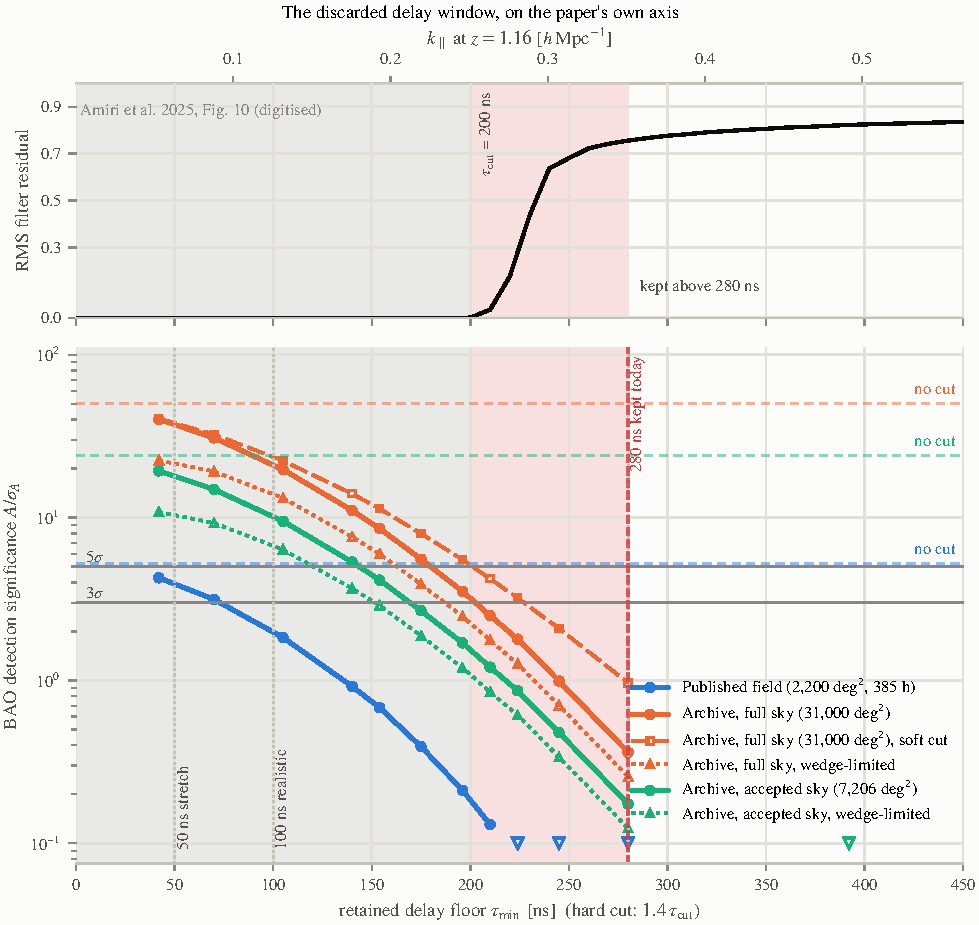
\includegraphics[width=0.80\textwidth]{fig_taucut_bao_fig10.pdf}
\caption{Forecast value of the discarded delay window, shown on the axis of Fig.~10 in~\cite[Sec.~5.3; Eq.~(37); Fig.~10]{chime2025auto}. \emph{Top:} published root-mean-square (RMS) filter residual as a function of mode delay, with the 200\,ns cut and 200--280\,ns recovery region shaded. \emph{Bottom:} BAO-amplitude detection significance from \texttt{RFIsher}, which uses RadioFisher's intensity-mapping Fisher matrix and BAO-amplitude formalism~\cite[Sec.~2.4, Eq.~(8), p.~5; Sec.~4.1, Eqs.~(13)--(14), Fig.~6, pp.~10--11; Sec.~4.2, Eqs.~(15)--(17), p.~11]{radiofisher}. The calculation and output are pinned to the cited revision~\cite[commit \texttt{c1302f44}; \protect\path{scripts/run_taucut_sweep.py}, lines~274--450; \protect\path{out/taucut_sweep.csv}, lines~22--28 and 86--113]{rfisher_code}. The forecast combines published field, band, and observing-time inputs~\cite[Abstract; Eq.~(46); Fig.~4]{chime2025auto} with the CHIME Overview instrument and noise model~\cite[Appendix~A; Table~2; Eq.~(A9)]{chime2022}. It adopts a retained delay floor $\tau_{\rm min}=1.4\,\tau_{\rm cut}$; the embedded 50 and 100\,ns annotations denote $\tau_{\rm min}$ on this axis. The published analysis has $\tau_{\rm min}=280$\,ns, where the forecast retains less than $0.01\sigma$ BAO sensitivity; open triangles mark values below the plot floor. Dotted curves retain the horizon wedge mask~\cite{seohirata2016}. Residual contamination is set to zero, so the figure measures the value of removed modes rather than leakage in retained modes. Table~\ref{tab:scen} states the assumptions for each curve.}
\label{fig:taucut}
\end{figure}

\subsection*{4. Feasibility and Preliminary Results}

\textbf{Forecast definition.} Figure~\ref{fig:taucut} reports $A/\sigma_A$, the forecast BAO-amplitude detection significance, as a function of the delay cut. I computed it with \texttt{RFIsher}, my Fisher framework based on RadioFisher's intensity-mapping and BAO formalism~\cite[Sec.~2.4, Eq.~(8), p.~5; Sec.~4.1, Eqs.~(13)--(14), Fig.~6, pp.~10--11; Sec.~4.2, Eqs.~(15)--(17), p.~11]{radiofisher}. The implementation and output are pinned to commit \texttt{c1302f44}~\cite[commit \texttt{c1302f44}; \path{scripts/run_taucut_sweep.py}, lines~274--450; \path{out/taucut_sweep.csv}, lines~22--28 and 86--113]{rfisher_code}. The 2025-field input case uses the published area, band, and observing time of 2,200\,deg$^2$, 608--708\,MHz, and 385\,h~\cite[Abstract; Eq.~(46); Fig.~4]{chime2025auto}, together with the CHIME Overview value $T_{\rm sys}=55$\,K~\cite[Appendix~A; Table~2; Eq.~(A9)]{chime2022}. The remaining cases use the seven-year archive over two possible sky areas.

\textbf{Forecast assumptions.} Table~\ref{tab:scen} separates the proposed deliverable from its external dependencies. This proposal delivers only a lower certified cut. Nearly seven years of archived observations and processing of the remaining lower-frequency band are separate collaboration efforts~\cite[Sec.~2.4; Sec.~3.2.1; Sec.~8]{chime2025auto}. The two archive rows bracket the largest remaining uncertainty, the usable sky area. To represent the empirical 280/200 recovery ratio in the current analysis~\cite[Sec.~5.3; Eq.~(64); Fig.~10]{chime2025auto}, the hard-cut forecast defines the retained delay floor as $\tau_{\rm min}=1.4\,\tau_{\rm cut}$. This relation is a modeling convention rather than a universal filter law. The soft-response variant applies the published response to the signal while leaving the noise unattenuated, so it is a conservative signal-only bound rather than a complete filtered-sensitivity model.

Residual contamination is set to zero. A total-power amplitude consistency check against the published $12.4\sigma$ result requires weaker small-scale damping than the RadioFisher fiducial, $\sigma_{\rm NL}=4.9$ rather than 7\,Mpc. This comparison is not a measurement of the instrumental noise. I retain the fiducial value; using the matched value would loosen the delay thresholds by 10--20\,ns. Three refinements remain. Baseline- and redshift-dependent cuts would increase the significance relative to a single global delay. Nonzero residual contamination \todo{run and add} would decrease it. If the wedge continues to set the cut on long baselines, reopening only short baselines reduces the significance by $0.7\times$ at every cut, as shown in the lower block of Table~\ref{tab:scen}. The quoted requirement is therefore an optimistic, zero-residual, global-cut bound.

\textbf{Forecast result.} At $\tau_{\rm cut}=125$\,ns on the Overview sky, the forecast gives $\sigma(\alpha_\parallel)=1.3\%$ and $\sigma(\alpha_\perp)=6.1\%$. The cut affects the radial and transverse scales differently.\par\pagebreak

Therefore, $H(z)\,r_d$ is the nearer-term product, while $D_A(z)/r_d$ requires a lower cut. The significance falls by a factor of 2.2 from 125 to 150\,ns, making the Year~2 milestone a numerical threshold. Increasing the accepted sky area can be as valuable as lowering the cut, which also motivates modeling leakage around bright sources instead of masking it.

\begin{table}[H]
\centering\footnotesize
\setlength{\tabcolsep}{3.5pt}
\renewcommand{\arraystretch}{1.15}
\begin{tabular}{@{}>{\raggedright\arraybackslash}p{3.15cm}>{\raggedright\arraybackslash}p{2.35cm}cccccc@{}}
\hline
Configuration & Assumes beyond this proposal & \multicolumn{4}{c}{$A/\sigma_A$ at $\tau_{\rm cut}$ [ns]} & \multicolumn{2}{c}{$\sigma(\alpha)$ at 150/125/100\,ns [\%]} \\
 & & 280 & 150 & 125 & 100 & $\alpha_\parallel$ & $\alpha_\perp$ \\
\hline
\multicolumn{8}{@{}l}{\emph{Canceller sets the cut on every baseline}} \\
Published-field inputs & none & 0.00 & 0.13 & 0.39 & 0.92 & --- & --- \\
Archive, accepted sky (7,206\,deg$^2$) & 7\,yr; full band & 0.00 & 1.21 & 2.68 & 5.34 & 5.4/2.7/1.5 & 35/13/5.1 \\
Archive, Overview sky (31,000\,deg$^2$) & 7\,yr; full band; $4.3\times$ sky & 0.01 & 2.50 & 5.55 & 11.1 & 2.6/1.3/0.74 & 17/6.1/2.5 \\
\hline
\multicolumn{8}{@{}l}{\emph{Wedge sets the cut on long baselines} (horizon wedge kept masked; baselines $<c\,\tau_{\rm cut}$ reopen)} \\
Published-field inputs & none & 0.00 & 0.09 & 0.28 & 0.65 & --- & --- \\
Archive, accepted sky (7,206\,deg$^2$) & 7\,yr; full band & 0.00 & 0.85 & 1.88 & 3.67 & 7.9/3.9/2.3 & 51/19/8.5 \\
Archive, Overview sky (31,000\,deg$^2$) & 7\,yr; full band; $4.3\times$ sky & 0.01 & 1.76 & 3.89 & 7.61 & 3.8/1.9/1.1 & 25/9.3/4.1 \\
\hline
\end{tabular}
\caption{Forecast scenarios for Fig.~\ref{fig:taucut}. The quantity $A/\sigma_A$ is the BAO-amplitude detection significance. The quantities $\sigma(\alpha_\parallel)$ and $\sigma(\alpha_\perp)$ are the fractional precisions of the radial and transverse dilation parameters. Residual contamination is set to zero throughout, and ``---'' denotes no detection at any listed cut. The lower block keeps the horizon wedge $\kpar<\kperp\,r(z)H(z)/[c(1+z)]$ masked~\cite{seohirata2016}. Lowering the cut then reopens only baselines shorter than $c\,\tau_{\rm cut}$, or 37\,m at 125\,ns; CHIME's longest east--west baseline is 66\,m, with $b/c=220$\,ns. The no-cut ceilings are 23 and 11$\sigma$, compared with 50 and 24$\sigma$ when the wedge is not retained. Only the lower cut is a deliverable of this proposal.}
\label{tab:scen}
\end{table}

\textbf{Controlled simulation.} The simulation in Fig.~\ref{fig:coh} evaluates Eq.~(\ref{eq:model}) using a delay-limited foreground coefficient of $10^4$ relative to the unit signal, white noise, and a visibility gain $g_ig_j^*$ with reflections at 33\,ns ($\epsilon=10^{-2}$) and 175\,ns ($3\times10^{-3}$). It contains 600 integrations at one declination. The reflections produce conjugate ridge pairs at $\Delta=\pm33$ and $\pm175$\,ns with $|\gamma|>0.98$. The ridge contrast, $\max_\tau|\gamma|/\mathrm{med}_\tau|\gamma|$, reaches approximately 20 at these delays over a floor of approximately 3. Smooth chromaticity with comparable root-mean-square amplitude gives a contrast of approximately 2.4 without isolated peaks.

The simulation gives two implementation requirements. First, the ridge locations form a difference set of the delay dictionary. The pair $(\tau,\Delta)$ helps identify physical delays, although the inverse mapping need not be unique. Second, an off-grid delay leaks across the delay axis as approximately $1/(\pi n)$ without apodization. A Blackman--Harris taper is therefore required. On the 2019 hybrid beamformed visibilities, the same map will provide the first decision gate. Isolated ridges would support a discrete-delay correction; broad structure would require a beam-model treatment; and a mixture would require both. In every case, the method will provide a measured reflection budget. \todo{Replace Fig.~\ref{fig:coh} with the real-data map when the requested 2019 data are in hand: recover the 33\,ns term, its phase against declination, detection significance and estimator variance, and the content of 110--300\,ns.}

\begin{figure}[t]
\centering
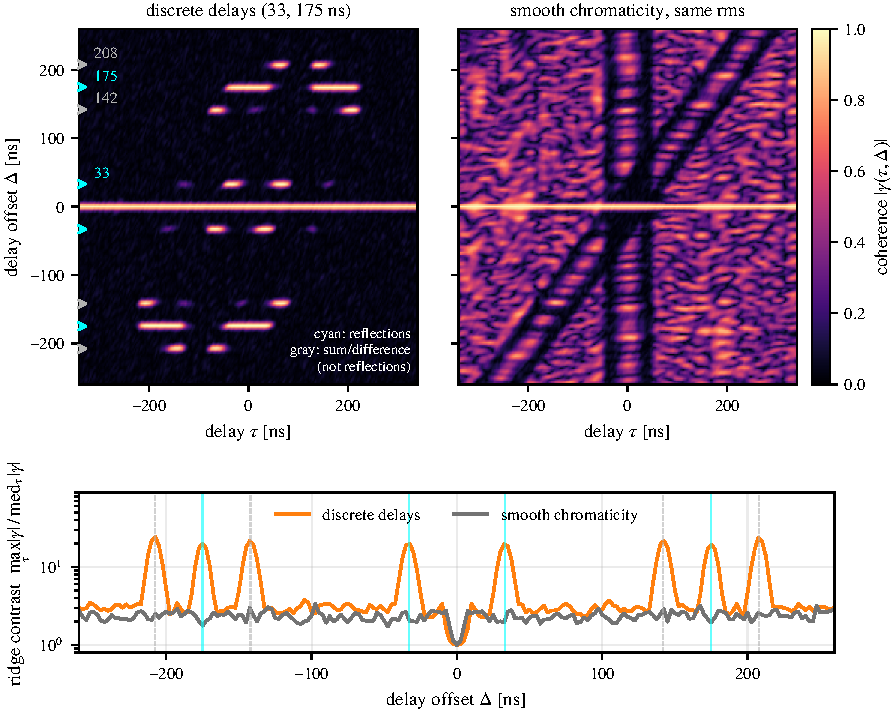
\includegraphics[width=0.92\textwidth]{fig_coherence_sim.pdf}
\caption{Simulated delay--offset coherence from Eq.~(\ref{eq:coh}). The top panels compare two discrete reflections (left) with smooth chromaticity of comparable root-mean-square amplitude (right). Cyan lines mark the physical reflection delays. Grey lines mark their sum and difference, which appear in the map but are not additional reflections. The bottom panel shows ridge contrast as a function of $\Delta$. Isolated peaks above a smooth floor are the feature tested by the real-data gate.}
\label{fig:coh}
\end{figure}

\textbf{Software and data access.} The estimator, survey, and forecasting components already exist as tested software in the WVURAIL GitHub organization: \texttt{pilot-proxy}, \texttt{RFIsher} with its RadioFisher fork, and the archive-survey layer in \texttt{datatrail}. CHIME collaboration membership is held by the individual rather than the institution, so my data access does not depend on the host. I am also integrating the pilot-proxy detector into \texttt{kotekan}, the real-time framework shared by CHIME and the Canadian Hydrogen Observatory and Radio-transient Detector (CHORD)~\cite{gormley2026c}. This integration provides the deployment path for the proposed estimator.

\subsection*{5. Work Plan}

\textbf{Year 1 --- gate, census, and estimator.}
\begin{itemize}
\item \emph{Gate (months 1--3).} I will compute the coherence map from the 2019 hybrid beamformed visibilities at several declinations on both sides of Cygnus~A. The statistical controls in Section~3, including the even--odd noise null, will set the detection threshold. Isolated ridges will support the hypothesis in Section~1 and define an initial dictionary. Broad structure, or a mixture of both signatures, will determine how much of Year~2 must combine the reflection census with the collaboration's beam model.
\item \emph{Census.} I will produce two data products because the archived visibilities average redundant baseline copies and do not retain feed indices. First, the per-feed census will use daily Cygnus~A gain solutions: 2048 inputs by 1024 channels per day, already archived, whose delay transforms directly contain each feed's reflections. Second, the per-baseline census will apply delay--offset coherence to redundancy-averaged visibilities for each polarization, east--west baseline, and declination over the seven-year archive. The outputs will report every detectable delay above the calibrated threshold, with amplitude and phase as functions of time, temperature, and calibration epoch. The 33\,ns standing wave is the validation case, and the 110--300\,ns population is the priority. The coherence statistic requires approximately $10^6$ operations per integration and channel set, so the analysis is expected to be limited by input/output (I/O) \todo{archive volume of the requested hybrid product, storage, and the named allocation}. This product is the instrument analogue of my dissertation's transmitter census and will support a separate publication.
\item \emph{Estimator.} I will apply the delay-shift canceller to the 2019 dataset using split-sample estimation and correction. I will report its false-alarm behavior, signal loss, and the corrected 100--280\,ns delay spectrum. The target residual will be consistent with noise plus the injected signal and contain no ridge above the calibrated threshold. As a safety milestone, I will reproduce the published $12.4\sigma$ result with the correction enabled and unchanged.
\end{itemize}
\textbf{Year 2, if the gate fails.} If broad chromaticity dominates instead of discrete ridges, I will use the census as a measured term in the collaboration's systematics budget. The per-feed gain-solution delays will become a calibration product, and I will apply the canceller to any discrete population that remains, with a separately certified $\tau_{\rm cut}$. The broad component provides a per-declination, per-baseline measurement of the chromatic beam's delay structure and will inform the holography-based beam model~\cite[Sec.~VI.3; Eqs.~(16)--(17); Figs.~16--17; Sec.~VII]{chime2024holo}. The milestone will be a per-baseline delay budget and a forecast of the cut it supports using the framework in Fig.~\ref{fig:taucut}.

\textbf{Year 2 --- lower the cut.} If the gate succeeds, I will lower $\tau_{\rm cut}$ on the full archive only as far as the certified residual permits. I will then measure the 21\,cm power spectrum in the newly available $\kpar$ bins using the collaboration's even/odd cross-spectrum and jackknife suite. The deliverable will be the first CHIME 21\,cm auto-spectrum at $z\simeq1$ below $\kpar=0.35\hMpc$, with every detected discrete delay included as a named term in the systematics budget. For the hard-cut forecast, the listed grid requires $\tau_{\rm cut}\le125$\,ns on the Overview sky and $\le100$\,ns when the accepted-sky mask is retained to exceed $5\sigma$. With the horizon wedge retained, the corresponding crossing lies in the 110--125\,ns interval for the Overview sky and the 75--100\,ns interval for the accepted sky. At 150\,ns, the fiducial full-sky hard-cut model gives $2.5\sigma$; the separately matched $\sigma_{\rm NL}=4.9$ model gives approximately $4.2\sigma$. I therefore treat 150\,ns as a model-dependent BAO-window measurement rather than a guaranteed detection, and use it as the fallback milestone.

\textbf{Year 3 --- BAO and transfer.} I will fit the BAO dilation parameter using the archive and the forecast-calibrated residual budget. The result will be either a constraint or a certified statement of the remaining requirement. I will also transfer the census and canceller to CHORD. Its 64-dish pathfinder is being commissioned, its 512-dish core is planned for completion at the end of 2027, and full-telescope commissioning is scheduled through 2028~\cite[Abstract, p.~2; Sec.~11, p.~18; Fig.~9, p.~19]{chord2026}. Subject to that published schedule, I will use pathfinder data in Year~1 and full-array data in Year~3. The dish--feed cavity will occur at a different delay, but the same physical model applies. I will also perform a cross-instrument test on a Kavli Institute for Cosmological Physics (KICP) spectrometer with a reflection cavity \todo{SPT-SLIM or TIM, per host}. Its etalon and filter-bank ripples provide the same periodic-in-frequency structure.

\subsection*{6. Risks}

\textbf{Discrete-delay hypothesis.} If smooth chromaticity dominates the window, I will deliver the measured reflection budget and combine it with the collaboration's beam model.

\textbf{Foreground wedge.} CHIME's 66\,m maximum east--west baseline has a horizon delay of approximately 220\,ns. Wedge contamination grows with baseline length and is not localized in $\Delta$. If it dominates, short baselines remain recoverable while long baselines stay masked. The lower block of Table~\ref{tab:scen} forecasts this case~\cite{seohirata2016}. At $z=1.16$, the wedge removes $\mu<0.61$, where $\mu$ is the line-of-sight direction cosine, and halves the no-cut ceiling. Reopened modes retain approximately $0.7\times$ their value, tightening the $5\sigma$ requirement by approximately 15\,ns to $\tau_{\rm cut}\simeq110$--$125$\,ns on the Overview sky and 75--100\,ns on the accepted sky.

\textbf{Steep threshold.} Increasing the cut from 125 to 150\,ns halves the forecast significance. I therefore treat 150\,ns as a fallback, not an assumed detection.

\textbf{Time-variable amplitudes.} Per-transit estimation is limited by $|\epsilon_k|^2P_F/P_N$ \todo{quantify from the coherence map}. I will pool weaker terms over one day and bound their drift from day-to-day differences.

\textbf{Filter mode coupling.} I will simulate the complete estimation and filtering chain, following the published analysis, and lower the cut only as far as its certified residual permits.

\textbf{Access after the move.} Collaboration membership is renewed by application and does not depend on the host \todo{confirm the renewal timeline and that the Canadian compute allocation travels with it}.

\subsection*{7. Broader Significance}

The proposed method applies to any spectrometer containing reflection cavities, cables, or coupled elements. These structures create discrete delays and force intensity-mapping analyses to discard low-$\kpar$ modes. CHIME combines a 21\,cm auto-spectrum detection at $z\simeq1$ with a seven-year archive, providing the data needed to develop and test the method. CHORD is a natural next application because its design emphasizes precise beam control and stable instrumental response~\cite[Abstract, p.~2; Sec.~1, pp.~2--3; Sec.~2.2, p.~4]{chord2026}. The same estimator can also support millimeter-wave line-intensity-mapping experiments by converting discrete instrumental delays into measured, testable terms in their systematics budgets. \todo{NHFP version: two sentences on relevance to NASA Astrophysics --- an independent BAO/growth probe at $1<z<2$, Roman's spectroscopic range, with disjoint systematics; and the applicant's intention to bring the method to NASA instrument pipelines.} \todo{KICP version: two sentences on fit --- dark energy from an independent tracer; systematics methodology shared with SPT-SLIM/TIM.}

% ------------------------------------------------------------------
\section*{Previous and Current Research}

For fifteen years, my research has focused on weak periodic structure in interference-limited radio environments. As a U.S.\ Army signals analyst from 2007 to 2012, false-alarm performance had direct operational consequences. At NASA Goddard from 2016 to 2017, I built FPGA back ends for the Wideband Radio-Frequency Interference (RFI) Mitigation testbed and implemented real-time spectral-kurtosis detection for spaceborne radiometry. At NASA Glenn from 2017 to 2022, I led cognitive-radio work for the Cognitive Communications Project. I held technical authority for real-time FPGA and software-defined-radio (SDR) systems supporting the Near Space Network and contributed core digital-signal-processing (DSP) engineering to the Space Communications and Navigation (SCaN) Testbed quantum-key-distribution emulation recognized by NASA Headquarters.

Cyclostationary signal processing connects this work. My 2021 M.S.\ thesis at Cleveland State developed a low-memory, streaming spectral-correlation analyzer for blind detection of digitally modulated waveforms~\cite[Abstract, p.~vii; Sec.~3.2, pp.~27--29]{gormley2021thesis}. I implemented this design on an FPGA as a spectrum sensor for CubeSat radios~\cite[Sec.~II; Figs.~7--9, p.~3; Sec.~III, Table~II, pp.~3--4]{gormley2021}, and then extended it using a hybrid memory--throughput architecture~\cite[pp.~34--36]{gormley2023}. I carried out this work in regular collaboration with C.~M.~Spooner, whose treatment of cyclic cumulants and spectral-correlation estimation underlies the proposed method. At AiRANACULUS from 2022 to 2023, I developed statistical detection and machine-learning methods for wideband radio-frequency sensing and interference mitigation~\cite[Sec.~IV, Figs.~5--6, pp.~3--4; Sec.~VI, Figs.~9 and 11, pp.~5--6]{mody2023a}. I also contributed to two NASA space-network resilience efforts~\cite[Secs.~III--V; Figs.~3--9, pp.~2--5]{mody2023b}. Related NASA cognitive-network research used the streaming spectrum sensor and radio-frequency-feature-enhanced architectures~\cite[Sec.~II.F, p.~272; Sec.~V, pp.~278--279]{dudukovich2022}.

\textbf{Dissertation: The Pilot-Proxy Method (WVU, defense spring 2027; advisor K.~Bandura).} The CHIME analysis detects and masks broadcast-television contamination~\cite[Sec.~3.1.2; Appendix~A.1, Eqs.~(A12)--(A15); Table~1]{chime2025auto}. Each ATSC waveform has a pilot carrier at a fixed offset, making it a proxy for the full 6\,MHz channel. This first-order periodic mean has a matched-filter $F$-statistic under the adopted tone and noise model, rather than a spectral-correlation detector. I implemented it as a bit-reproducible, fixed-point graphics-processing-unit (GPU) pipeline and surveyed the baseband archive with per-epoch calibration measured from the data~\cite{gormley2026a}. The survey layer is now part of \texttt{datatrail}.

Three dissertation results support the proposed work. First, I derived the masking-scaling relation for a sidereal stack. The sky signal and constant terrestrial interference are both coherent, so unmasked channels approach an interference-bias floor instead of BAO depth. If $\eta$ is the retained fraction and $T$ is the observing time, masking restores the noise-limited $1/\sqrt{\eta T}$ scaling at a $1/\eta$ cost in elapsed observing time. A canary bound on sub-threshold leakage tests this result. Second, I set per-channel thresholds from the science requirement rather than the detector floor. A null-bulk calibration fixes the false-alarm probability, and \texttt{RFIsher} expresses the threshold in integration-time cost and BAO parameter bias~\cite{gormley2026b}. Third, I produced a feed-by-feed census of digital-television (DTV) transmitters around the observatory. \todo{Add three headline numbers: detection depth relative to the noise floor, false-alarm rate achieved, and archive volume surveyed.} I am currently integrating the detector into the \texttt{kotekan} framework shared by CHIME and CHORD~\cite{gormley2026c}.

\textbf{Leadership and community.} At NASA Glenn, I led the Cognitive Communications team and mentored interns and new-hire engineers. I have served as a session chair and reviewer for the Institute of Electrical and Electronics Engineers (IEEE) Cognitive Communications for Aerospace Applications Workshop, reviewed for IEEE MILCOM, and reviewed NASA Small Business Innovation Research proposals. I have served as a teaching assistant in circuit theory, digital signal processing, software-defined radio, and senior capstone, and participated in NASA outreach. At WVU, I help manage the DSPIRA program, which teaches signal processing through radio astronomy; my role is programmatic rather than classroom-based.

The proposed work follows directly from these results. It applies the second-order estimator developed during my M.S.\ and NASA research, together with the validation methods and data pipelines from my dissertation, to periodic structure produced by the instrument itself.

% ------------------------------------------------------------------
\begin{thebibliography}{99}\small
\bibitem{desi2024} DESI Collaboration, ``DESI 2024 VI: Cosmological constraints from the measurements of baryon acoustic oscillations,'' arXiv:2404.03002 (2024).
\bibitem{chime2022} CHIME Collaboration, ``An overview of CHIME, the Canadian Hydrogen Intensity Mapping Experiment,'' ApJS 261, 29 (2022).
\bibitem{roman2021} Y.~Wang et al., ``The High Latitude Spectroscopic Survey on the Nancy Grace Roman Space Telescope,'' ApJ 928, 1 (2022), arXiv:2110.01829.
\bibitem{chime2023} CHIME Collaboration, ``Detection of cosmological 21 cm emission with the Canadian Hydrogen Intensity Mapping Experiment,'' ApJ 947, 16 (2023).
\bibitem{chime2024lya} CHIME Collaboration, ``A detection of cosmological 21 cm emission from CHIME in cross-correlation with eBOSS measurements of the Lyman-$\alpha$ forest,'' ApJ (2024), doi:10.3847/1538-4357/ad0f1d.
\bibitem{chime2025auto} CHIME Collaboration, ``Detection of the cosmological 21 cm signal in auto-correlation at $z\sim1$ with the Canadian Hydrogen Intensity Mapping Experiment,'' arXiv:2511.19620 (2025).
\bibitem{chime2024holo} CHIME Collaboration, ``Holographic beam measurements of the Canadian Hydrogen Intensity Mapping Experiment,'' ApJ (2024), doi:10.3847/1538-4357/ad8133.
\bibitem{dayenu} A.~Ewall-Wice et al., ``DAYENU: a simple filter of smooth foregrounds for intensity mapping power spectra,'' MNRAS 500, 5195 (2021).
\bibitem{hyfores} H.~Wang, K.~Masui, K.~Bandura, A.~Chakraborty et al., ``Demonstration of hybrid foreground removal on CHIME data,'' Phys.\ Rev.\ D 111, 103531 (2025), arXiv:2408.08949.
\bibitem{hyfores_sim} H.~Wang, P.~Phoompuang, K.~W.~Masui, A.~Chakraborty and S.~Foreman, ``Mitigating antenna gain errors with hybrid foreground residual subtraction in CHIME simulations,'' Phys.\ Rev.\ D 113, 043550 (2026).
\bibitem{kern2019} N.~S.~Kern et al., ``Mitigating internal instrument coupling for 21 cm cosmology. I. Temporal and spectral modeling in simulations,'' ApJ 884, 105 (2019).
\bibitem{kern2020} N.~S.~Kern et al., ``Mitigating internal instrument coupling for 21 cm cosmology. II. A method demonstration with HERA,'' ApJ 888, 70 (2020).
\bibitem{gardner2006} W.~A.~Gardner, A.~Napolitano and L.~Paura, ``Cyclostationarity: Half a century of research,'' Signal Processing 86, 639 (2006).
\bibitem{tong1994} L.~Tong, G.~Xu and T.~Kailath, ``Blind identification and equalization based on second-order statistics: a time domain approach,'' IEEE Trans.\ Inf.\ Theory 40, 340 (1994).
\bibitem{radiofisher} P.~Bull, P.~G.~Ferreira, P.~Patel and M.~G.~Santos, ``Late-time cosmology with 21 cm intensity mapping experiments,'' ApJ 803, 21 (2015).
\bibitem{seohirata2016} H.-J.~Seo and C.~M.~Hirata, ``The foreground wedge and 21-cm BAO surveys,'' MNRAS 456, 3142 (2016).
\bibitem{chord2026} CHORD Collaboration, ``Overview of the Canadian Hydrogen Observatory and Radio Transient Detector (CHORD) project,'' arXiv:2607.09374 (2026).
\bibitem{rfisher_code} D.~J.~Gormley, \texttt{RFIsher}: noise-tolerance forecasting for 21\,cm surveys, commit \texttt{c1302f44}, \url{https://github.com/WVURAIL/RFIsher/tree/c1302f441949e6d3f152a28687e4cf39c8cbd656} (2026).
\bibitem{gormley2026a} D.~J.~Gormley and K.~Bandura, ``The Pilot-Proxy Method: Digital-television RFI detection and BAO noise tolerance in CHIME,'' in preparation (2026).
\bibitem{gormley2026b} D.~J.~Gormley and K.~Bandura, ``Noise-tolerance forecasting for radio-telescope back-ends with application to 21-cm BAO surveys,'' in preparation (2026).
\bibitem{gormley2026c} D.~J.~Gormley, K.~Bandura et al.\ (CHIME Collaboration), ``Pilot-proxy RFI excision in the CHIME and CHORD pipelines,'' in preparation (2026).
\bibitem{gormley2023} D.~J.~Gormley, ``A hybrid technique to increase throughput of the streaming spectrum sensor,'' Proc.\ IEEE SHaRC, 34--36 (2023).
\bibitem{gormley2021} D.~J.~Gormley et al., ``A spectrum sensor for CubeSat radios,'' Proc.\ IEEE CCAAW, 1--5 (2021).
\bibitem{gormley2021thesis} D.~J.~Gormley, ``A low-memory spectral-correlation analyzer for digital QAM-SRRC waveforms,'' M.S.\ thesis, Cleveland State University (2021).
\bibitem{mody2023a} A.~N.~Mody et al., ``CLAIRE: Enabling heterogeneous communication network optimization for robust and resilient operations,'' Proc.\ IEEE CCAAW, 1--6 (2023).
\bibitem{mody2023b} A.~N.~Mody et al., ``INSPiRE: An approach to mission quality management using network slicing for space applications,'' Proc.\ IEEE CCAAW, 1--6 (2023).
\bibitem{dudukovich2022} R.~Dudukovich, D.~J.~Gormley et al., ``Toward the development of a multi-agent cognitive networking system for the lunar environment,'' IEEE J.\ Radio Freq.\ Identification 6, 269--283 (2022).
\end{thebibliography}

\end{document}
